\documentclass{article}

\begin{document}

\setlength{\parindent}{6ex}

\begin{figure}
    \centering
    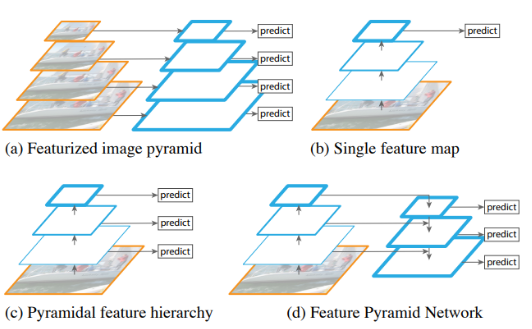
\includegraphics[width=0.75\textwidth]{multiscalefeatmaps}
    \caption{Different methods to use feature maps}
    \label{fig:multiscalefeatmaps1}
\end{figure}

\indent

Multi-scale handling refers to detect objects that have different 
sizes in a given frame. Multi-scale handling is a crucial feature for 
having a well performing detector since most of the objects in images
have different sizes. There are various ways to handle this problem: \par

One of the solutions (Fig. \ref{fig:multiscalefeatmaps1}(a)) is to run detection multiple times that in each 
run, the resolution of the input frame has to be changed. Then, all the 
detected objects have to be combined after all iterations are completed. 
In the case of multiple detections for the same object, a suppression has to be 
performed to reduce single detection. Although this method works well, 
its runtime is slow. \par

Another solution (Fig. \ref{fig:multiscalefeatmaps1}(b)) is to use single feature map. In this method, a single 
feature map is extracted from given frame and this feature map is passed 
through multiple convolutional layers to obtain a final feature map with 
more fine-grained features. Then, this feature map is used to predict the 
objects in the given frame. This method is used to obtain fast detection but 
its performance is relatively worse than other methods. \par

Another solution (Fig. \ref{fig:multiscalefeatmaps1}(c)) is to use a pyramidal feature hierarchy in which multiple 
feature maps are used to make a prediction. In this method, a feature map 
is extracted from the given frame and as it is in the second solution, this 
feature map is passed through multiple convolutional layers. However, 
in each layer, the extracted feature map is used to make a prediction. This 
method is relatively slower than the second solution but it performs better. \par

Another solution (Fig. \ref{fig:multiscalefeatmaps1}(d)) is to use feature pyramid network but this method will be 
examined in section 3.2.6. 
\end{document}